% Week 57 / Area from dots / K-1 student pages (packet N57-K-v1), revised
% after review.md and review-math.md.
% Compile with xelatex (or lualatex). All working boards use x = y = 20 mm so
% the kit's 20 mm squares and halves sit on the dots when printed at 100%.
% The p. 1 convention row and launch strip are illustrations at 12 mm.
\documentclass[12pt]{article}
\usepackage[letterpaper,left=15mm,right=15mm,top=12mm,bottom=12mm,
  headheight=6mm,headsep=6mm,footskip=10mm,includehead,includefoot]{geometry}
\usepackage{fontspec}
\setmainfont{TeX Gyre Heros}
\usepackage{fancyhdr}
\usepackage{tikz}
\usetikzlibrary{arrows.meta,calc,shapes.geometric}

\pagestyle{fancy}
\fancyhf{}
\fancyhead[L]{Week 57 / Area from dots / K–1}
\fancyfoot[L]{\small Bellingham Math Circle / Week 57 / N57-K-v1}
\fancyfoot[R]{\small \thepage}
\renewcommand{\headrulewidth}{0.4pt}
\renewcommand{\footrulewidth}{0pt}

\setlength{\parindent}{0pt}
\setlength{\parskip}{0pt}
\linespread{1.12}

\newcommand{\prob}[1]{\textbf{Problem #1:}}

% ---------- drawing helpers (inside a picture with x = y = 20 mm) ----------
\newcommand{\dotrad}{1.3mm}
% \grid{x0}{y0}{nx}{ny}: nx by ny dots, bottom-left dot at (x0,y0)
\newcommand{\grid}[4]{%
  \foreach \i in {1,...,#3}{\foreach \j in {1,...,#4}{%
    \fill ({#1+\i-1},{#2+\j-1}) circle (\dotrad);}}}
% \frm{x0}{y0}{nx}{ny}: light frame around a board of nx by ny dots
\newcommand{\frm}[4]{%
  \draw[gray!65,line width=0.5pt,rounded corners=2.5mm]
    ({#1-0.22},{#2-0.22}) rectangle ({#1+#3-1+0.22},{#2+#4-1+0.22});}
\newcommand{\board}[4]{\frm{#1}{#2}{#3}{#4}\grid{#1}{#2}{#3}{#4}}
% marks
\newcommand{\cmark}[1]{\draw[line width=0.75pt] (#1) circle (3.3mm);}
\newcommand{\bmark}[1]{\draw[line width=0.75pt] ($(#1)+(-3.2mm,-3.2mm)$) rectangle ($(#1)+(3.2mm,3.2mm)$);}
% target dot: a filled star drawn over the dot, centred on it
\newcommand{\stardot}[1]{\node[star,star points=5,star point ratio=2.3,fill=black,
  draw=none,inner sep=0pt,minimum size=6.2mm] at (#1) {};}
% record icons; #1 = left end of the group (x,y)
\newcommand{\halfic}[1]{%
  \filldraw[fill=gray!35,line width=0.5pt] ($(#1)+(0,-2.2mm)$) -- ++(4.6mm,0) -- ++(-4.6mm,4.6mm) -- cycle;
  \draw[line width=0.5pt] ($(#1)+(6.6mm,-2.2mm)$) -- ++(13mm,0);}
\newcommand{\circic}[1]{%
  \fill ($(#1)+(2.3mm,0)$) circle (0.9mm);
  \draw[line width=0.6pt] ($(#1)+(2.3mm,0)$) circle (2.3mm);
  \draw[line width=0.5pt] ($(#1)+(6.6mm,-2.2mm)$) -- ++(13mm,0);}
% a written entry on a record blank whose icon group starts at #1
\newcommand{\recval}[2]{\node[anchor=base,font=\large] at ($(#1)+(13.1mm,-1.2mm)$) {#2};}
% centred record rows under a board: centre (cx,cy)
\newcommand{\recC}[2]{\circic{{#1-0.49},{#2}}}
\newcommand{\recHC}[2]{\halfic{{#1-1.08},{#2}}\circic{{#1+0.10},{#2}}}

% yes / no marks for the convention pictures, centred at #1
\newcommand{\yesmark}[1]{\draw[line width=1.6pt] ($(#1)+(-2.6mm,0.2mm)$) -- ++(1.9mm,-2.3mm) -- ++(3.6mm,4.8mm);}
\newcommand{\nomark}[1]{\draw[line width=1.6pt] ($(#1)+(-2.2mm,-2.2mm)$) -- ++(4.4mm,4.4mm)
  ($(#1)+(-2.2mm,2.2mm)$) -- ++(4.4mm,-4.4mm);}

\tikzset{every picture/.style={line cap=round,line join=round}}
\newcommand{\shapefill}{gray!14}
\newcommand{\piecefill}{gray!35}

\begin{document}

% ============================== PAGE 1 ==============================
Squares and halves go flat on the dots, with every corner on a dot. Pieces
join along whole sides into one shape, with no gap inside. A square counts as
two halves. Circle the dots on the outline of a shape and box the dots inside
it.

\vspace{4mm}
% ---- convention row (12 mm scale): side join yes, corner touch no, square = two halves
\noindent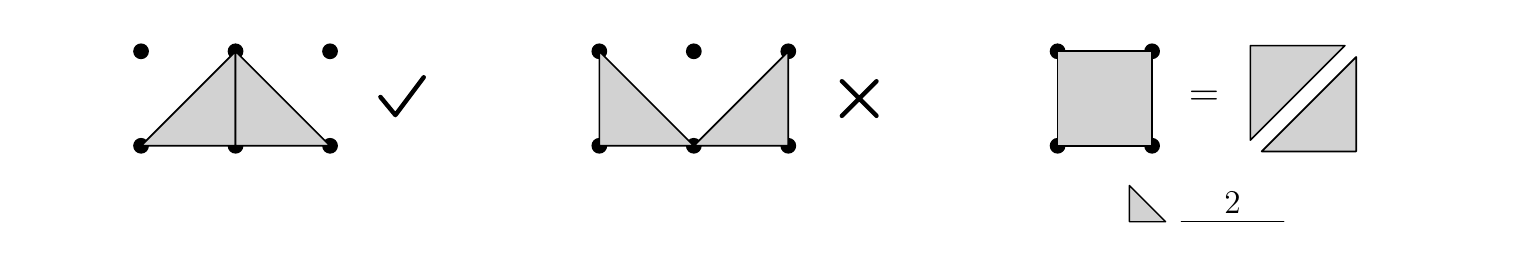
\begin{tikzpicture}[x=12mm,y=12mm]
  \useasboundingbox (0,-1.05) rectangle (15.49,1.25);
  % yes: two halves joined along a whole side
  \begin{scope}[shift={(1.2,0)}]
    \foreach \i in {0,1,2}{\foreach \j in {0,1}{\fill (\i,\j) circle (1mm);}}
    \filldraw[fill=\piecefill,line width=0.6pt] (0,0) -- (1,0) -- (1,1) -- cycle;
    \filldraw[fill=\piecefill,line width=0.6pt] (1,0) -- (2,0) -- (1,1) -- cycle;
    \yesmark{2.75,0.5}
  \end{scope}
  % no: two halves touching only at a corner
  \begin{scope}[shift={(6.05,0)}]
    \foreach \i in {0,1,2}{\foreach \j in {0,1}{\fill (\i,\j) circle (1mm);}}
    \filldraw[fill=\piecefill,line width=0.6pt] (0,0) -- (1,0) -- (0,1) -- cycle;
    \filldraw[fill=\piecefill,line width=0.6pt] (1,0) -- (2,0) -- (2,1) -- cycle;
    \nomark{2.75,0.5}
  \end{scope}
  % a square counts as two halves
  \begin{scope}[shift={(10.9,0)}]
    \foreach \i in {0,1}{\foreach \j in {0,1}{\fill (\i,\j) circle (1mm);}}
    \filldraw[fill=\piecefill,line width=0.6pt] (0,0) rectangle (1,1);
    \node[font=\Large] at (1.55,0.5) {=};
    % two loose halves, pulled slightly apart so both pieces show
    \filldraw[fill=\piecefill,line width=0.6pt] (2.16,-0.06) -- (3.16,-0.06) -- (3.16,0.94) -- cycle;
    \filldraw[fill=\piecefill,line width=0.6pt] (2.04,0.06) -- (3.04,1.06) -- (2.04,1.06) -- cycle;
  \end{scope}
  \halfic{{11.66},{-0.62}}
  \recval{11.66,-0.62}{2}
\end{tikzpicture}

\vspace{5mm}
% ---- launch strip (12 mm scale): pieces on dots -> outline traced -> dots marked
\noindent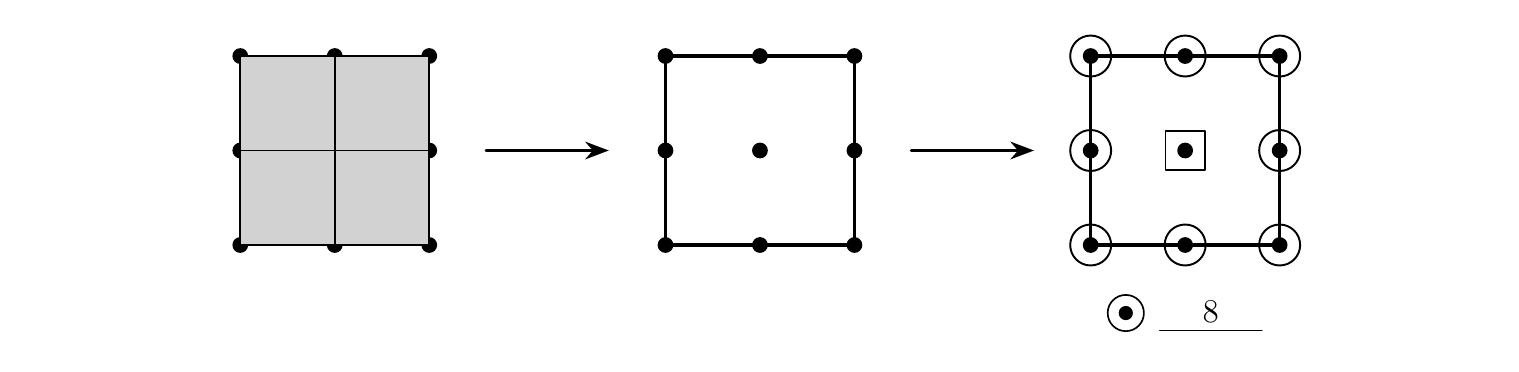
\begin{tikzpicture}[x=12mm,y=12mm]
  \useasboundingbox (0,-1.05) rectangle (15.49,2.3);
  % panel A: four squares on the dots
  \begin{scope}[shift={(2.25,0)}]
    \foreach \i in {0,1,2}{\foreach \j in {0,1,2}{\fill (\i,\j) circle (1mm);}}
    \foreach \i/\j in {0/0,1/0,0/1,1/1}{
      \filldraw[fill=\piecefill,line width=0.6pt] (\i,\j) rectangle ++(1,1);}
  \end{scope}
  \draw[-{Stealth[length=3mm]},line width=0.9pt] (4.85,1) -- (6.15,1);
  % panel B: outline drawn, pieces lifted
  \begin{scope}[shift={(6.75,0)}]
    \draw[line width=1.2pt] (0,0) rectangle (2,2);
    \foreach \i in {0,1,2}{\foreach \j in {0,1,2}{\fill (\i,\j) circle (1mm);}}
  \end{scope}
  \draw[-{Stealth[length=3mm]},line width=0.9pt] (9.35,1) -- (10.65,1);
  % panel C: outline dots circled, inside dot boxed, and its outline record
  \begin{scope}[shift={(11.25,0)}]
    \draw[line width=1.2pt] (0,0) rectangle (2,2);
    \foreach \i in {0,1,2}{\foreach \j in {0,1,2}{\fill (\i,\j) circle (1mm);}}
    \foreach \p in {(0,0),(1,0),(2,0),(2,1),(2,2),(1,2),(0,2),(0,1)}{
      \draw[line width=0.7pt] \p circle (2.6mm);}
    \draw[line width=0.7pt] ($(1,1)+(-2.5mm,-2.5mm)$) rectangle ($(1,1)+(2.5mm,2.5mm)$);
    \circic{{0.18},{-0.72}}
  \end{scope}
  \recval{11.43,-0.72}{8}
\end{tikzpicture}

\vspace{6mm}
\prob{1} Cover each shape with halves.

\vspace{5mm}
\noindent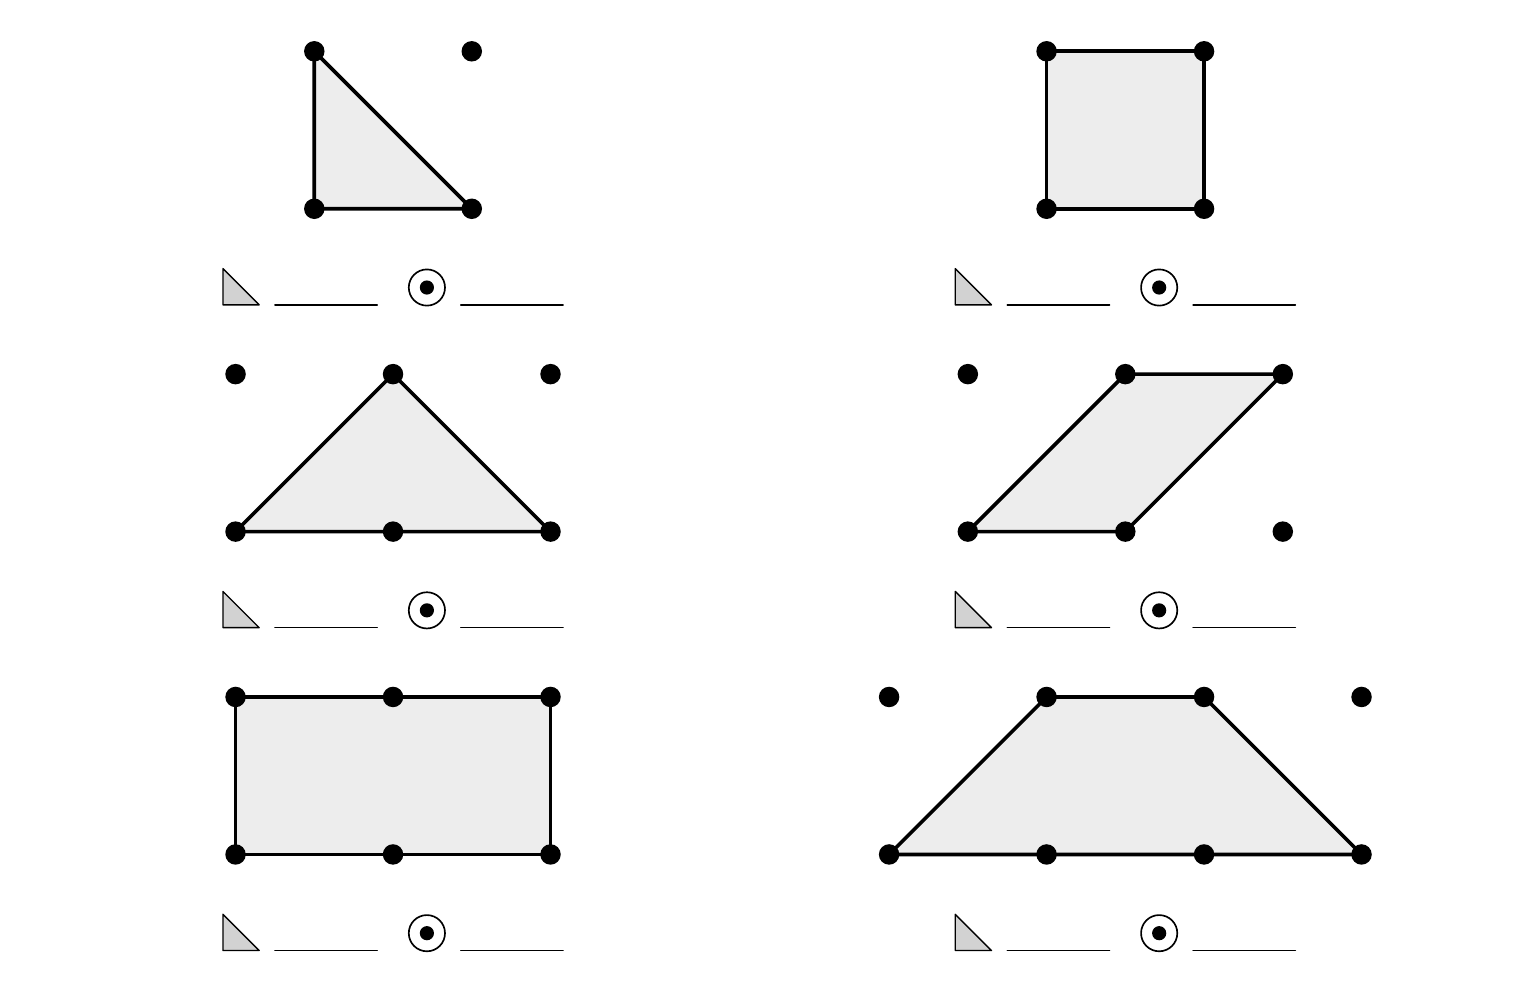
\begin{tikzpicture}[x=20mm,y=20mm]
  \useasboundingbox (0,-4.82) rectangle (9.295,1.15);
  % row 1: one half; a square
  \begin{scope}[shift={(1.82,0)}]
    \filldraw[fill=\shapefill,line width=1.3pt] (0,0) -- (1,0) -- (0,1) -- cycle;
    \grid{0}{0}{2}{2}
  \end{scope}
  \recHC{2.32}{-0.5}
  \begin{scope}[shift={(6.47,0)}]
    \filldraw[fill=\shapefill,line width=1.3pt] (0,0) rectangle (1,1);
    \grid{0}{0}{2}{2}
  \end{scope}
  \recHC{6.97}{-0.5}
  % row 2: two slanted shapes of two halves
  \begin{scope}[shift={(1.32,-2.05)}]
    \filldraw[fill=\shapefill,line width=1.3pt] (0,0) -- (2,0) -- (1,1) -- cycle;
    \grid{0}{0}{3}{2}
  \end{scope}
  \recHC{2.32}{-2.55}
  \begin{scope}[shift={(5.97,-2.05)}]
    \filldraw[fill=\shapefill,line width=1.3pt] (0,0) -- (1,0) -- (2,1) -- (1,1) -- cycle;
    \grid{0}{0}{3}{2}
  \end{scope}
  \recHC{6.97}{-2.55}
  % row 3: two shapes of four halves
  \begin{scope}[shift={(1.32,-4.1)}]
    \filldraw[fill=\shapefill,line width=1.3pt] (0,0) rectangle (2,1);
    \grid{0}{0}{3}{2}
  \end{scope}
  \recHC{2.32}{-4.6}
  \begin{scope}[shift={(5.47,-4.1)}]
    \filldraw[fill=\shapefill,line width=1.3pt] (0,0) -- (3,0) -- (2,1) -- (1,1) -- cycle;
    \grid{0}{0}{4}{2}
  \end{scope}
  \recHC{6.97}{-4.6}
\end{tikzpicture}

\newpage
% ============================== PAGE 2 ==============================
\prob{2} Make shapes from three halves, one on each board. Can you make two
shapes with different numbers of dots on their outlines?

\vspace{6mm}
\noindent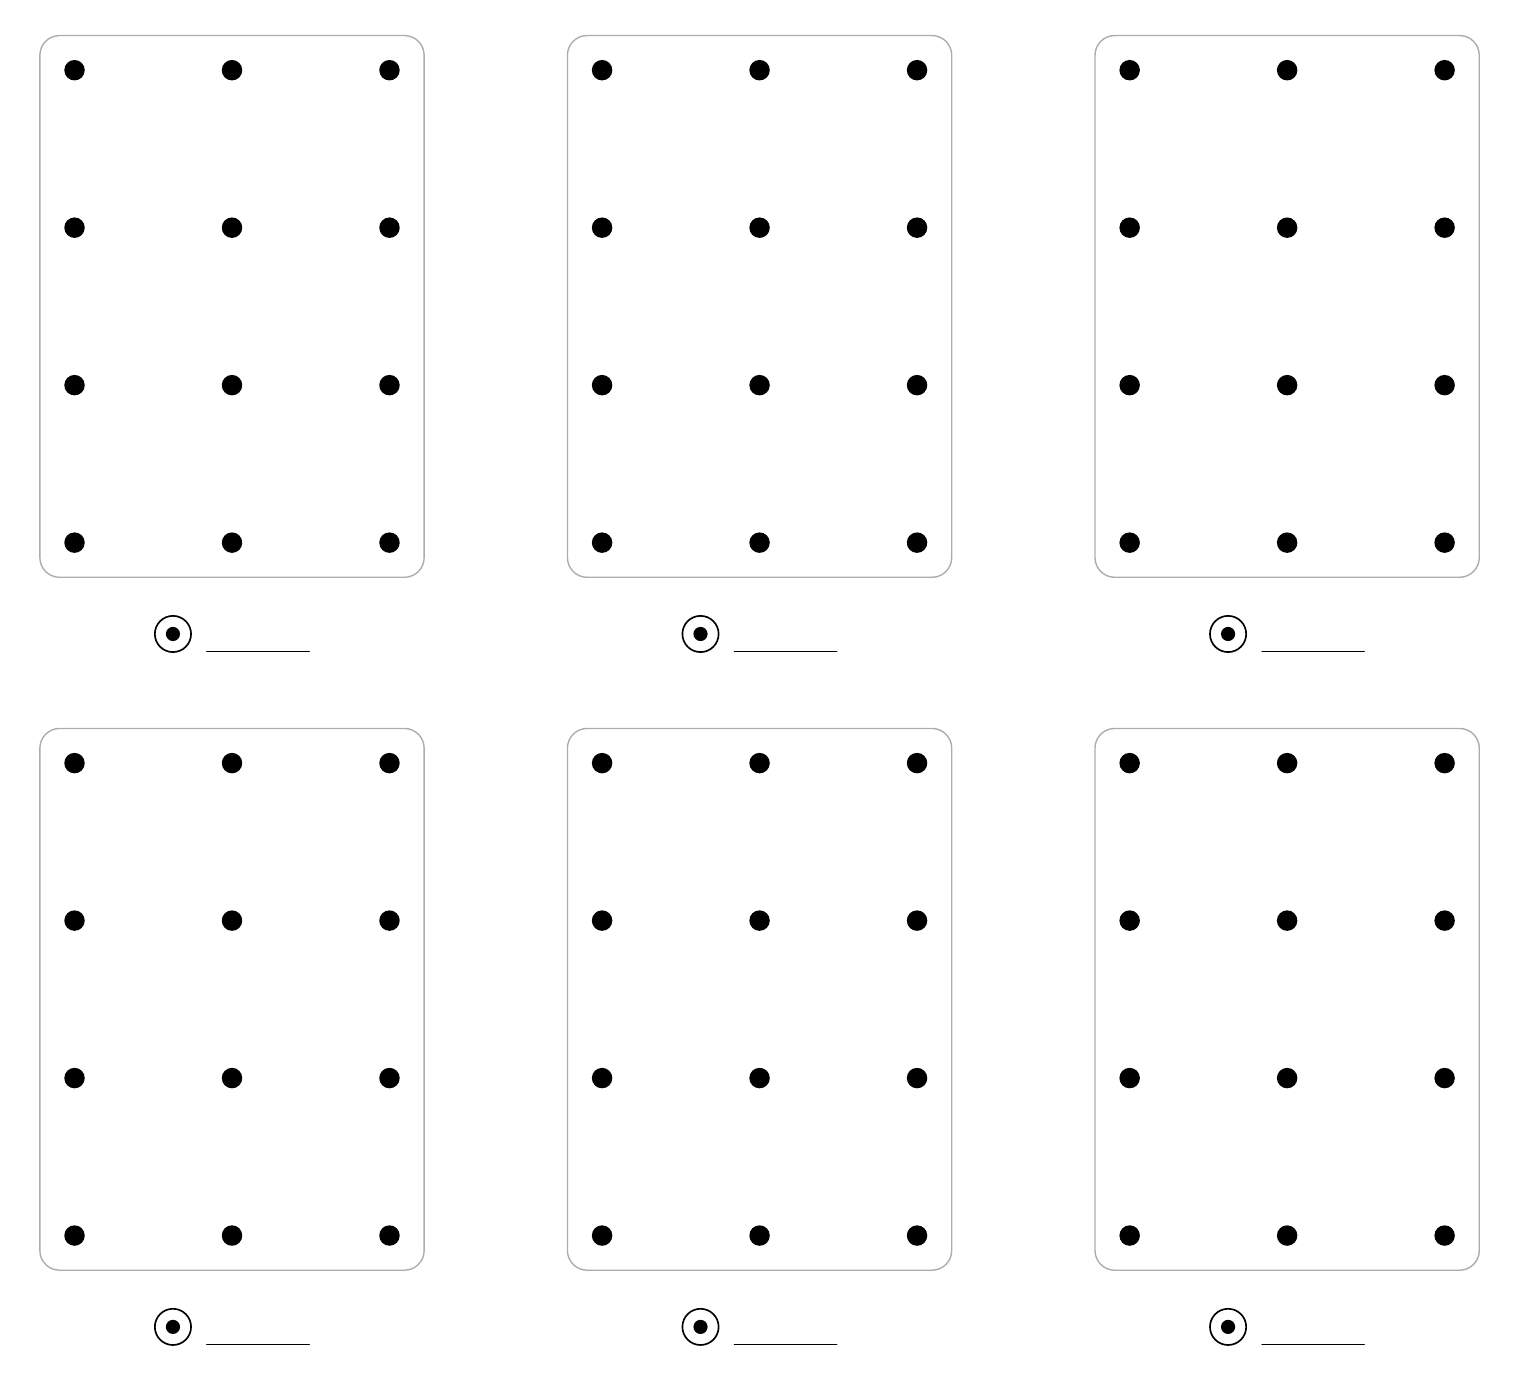
\begin{tikzpicture}[x=20mm,y=20mm]
  \useasboundingbox (0,-8.45) rectangle (9.295,0.05);
  \foreach \c in {0,1,2}{
    \pgfmathsetmacro{\xl}{0.2975+\c*3.35}
    \board{\xl}{-3.22}{3}{4}
    \recC{\xl+1}{-3.8}
    \board{\xl}{-7.62}{3}{4}
    \recC{\xl+1}{-8.2}
  }
\end{tikzpicture}

\newpage
% ============================== PAGE 3 ==============================
\prob{3} Make different shapes from four halves, one on each board. Find one
with as few dots on its outline as you can.

\vspace{6mm}
\noindent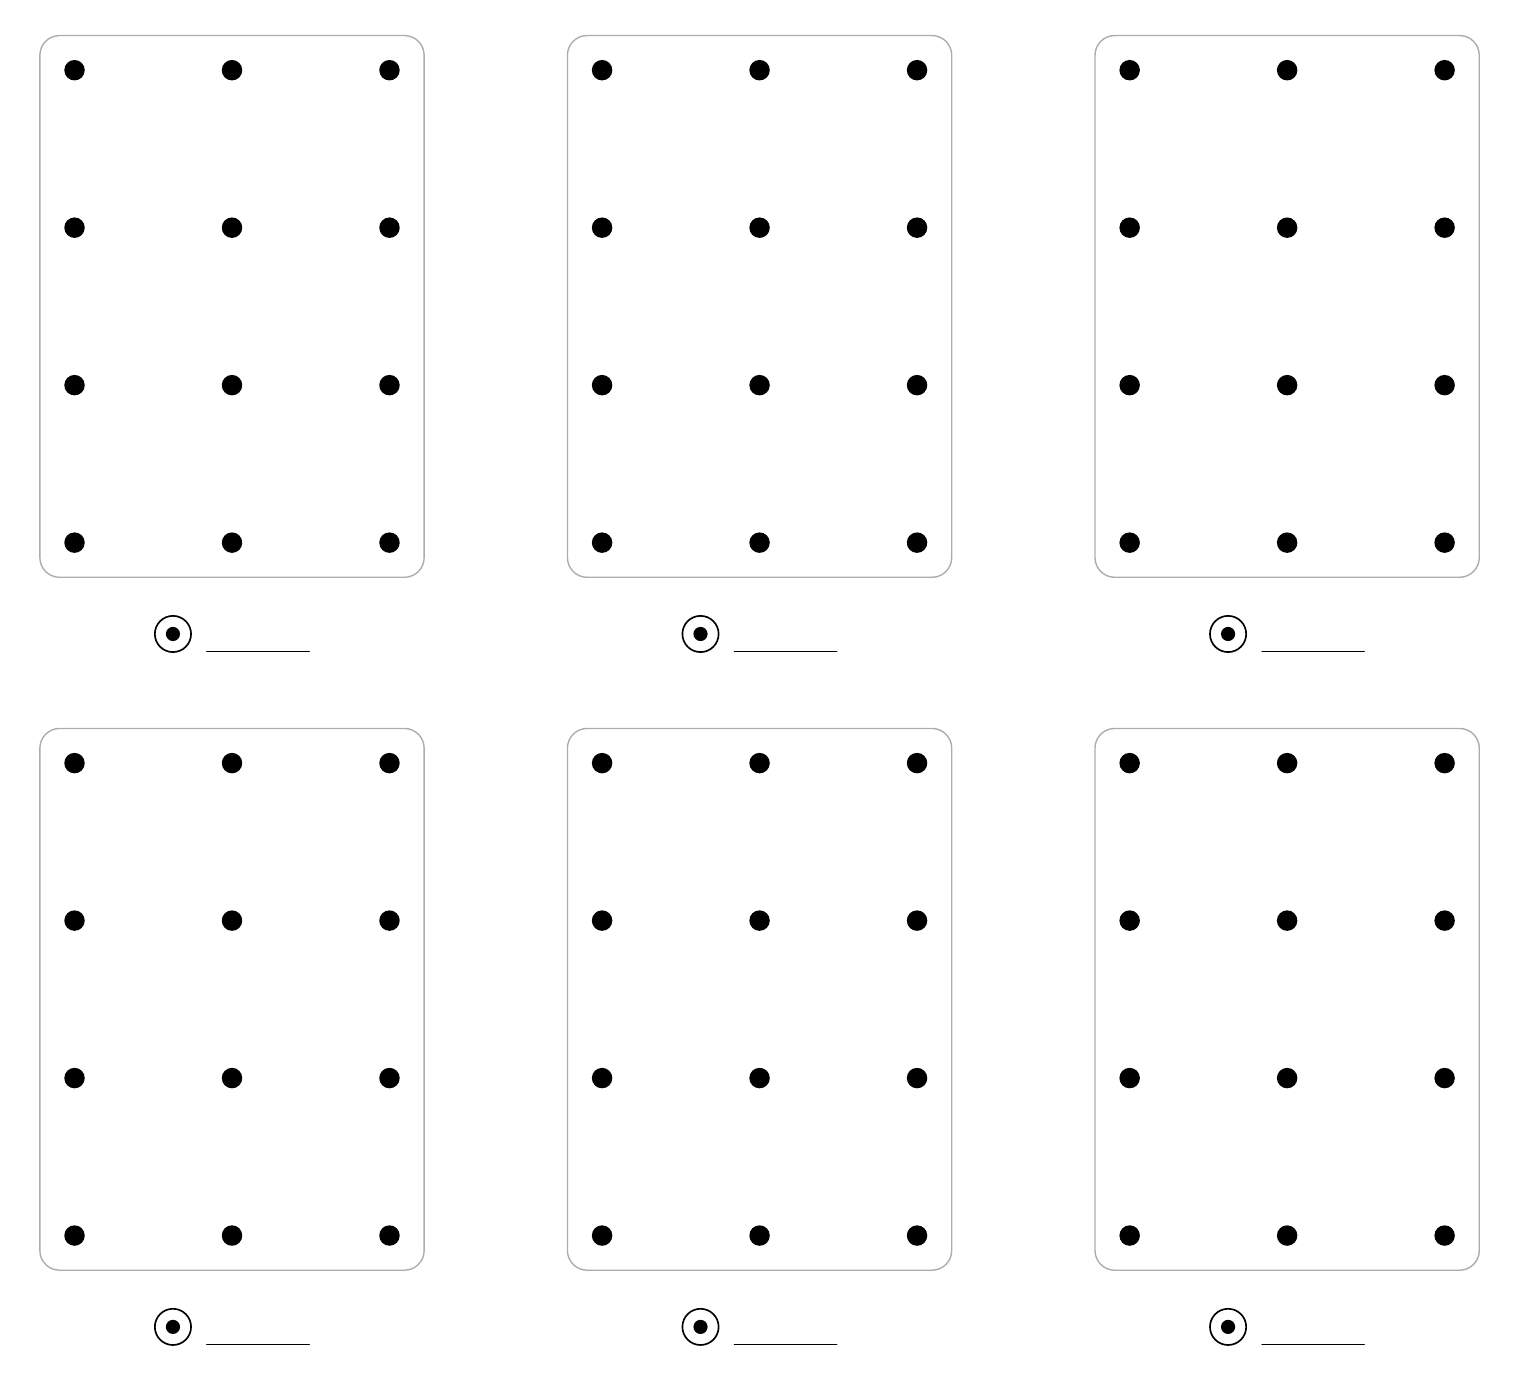
\begin{tikzpicture}[x=20mm,y=20mm]
  \useasboundingbox (0,-8.45) rectangle (9.295,0.05);
  \foreach \c in {0,1,2}{
    \pgfmathsetmacro{\xl}{0.2975+\c*3.35}
    \board{\xl}{-3.22}{3}{4}
    \recC{\xl+1}{-3.8}
    \board{\xl}{-7.62}{3}{4}
    \recC{\xl+1}{-8.2}
  }
\end{tikzpicture}

\newpage
% ============================== PAGE 4 ==============================
\prob{4} Can three pieces make a shape with the star inside? If they can, make
one. If they can't, explain why.

\vspace{6mm}
\noindent\begin{tikzpicture}[x=20mm,y=20mm]
  \useasboundingbox (0,-0.25) rectangle (9.295,4.25);
  \board{2.6475}{0}{5}{5}
  \stardot{4.6475,2}
\end{tikzpicture}

\newpage
% ============================== PAGE 5 ==============================
\prob{5} Make shapes from four pieces with the star inside, one on each board.
A turned shape counts as the same shape. How many different shapes can you
find?

\vspace{6mm}
\noindent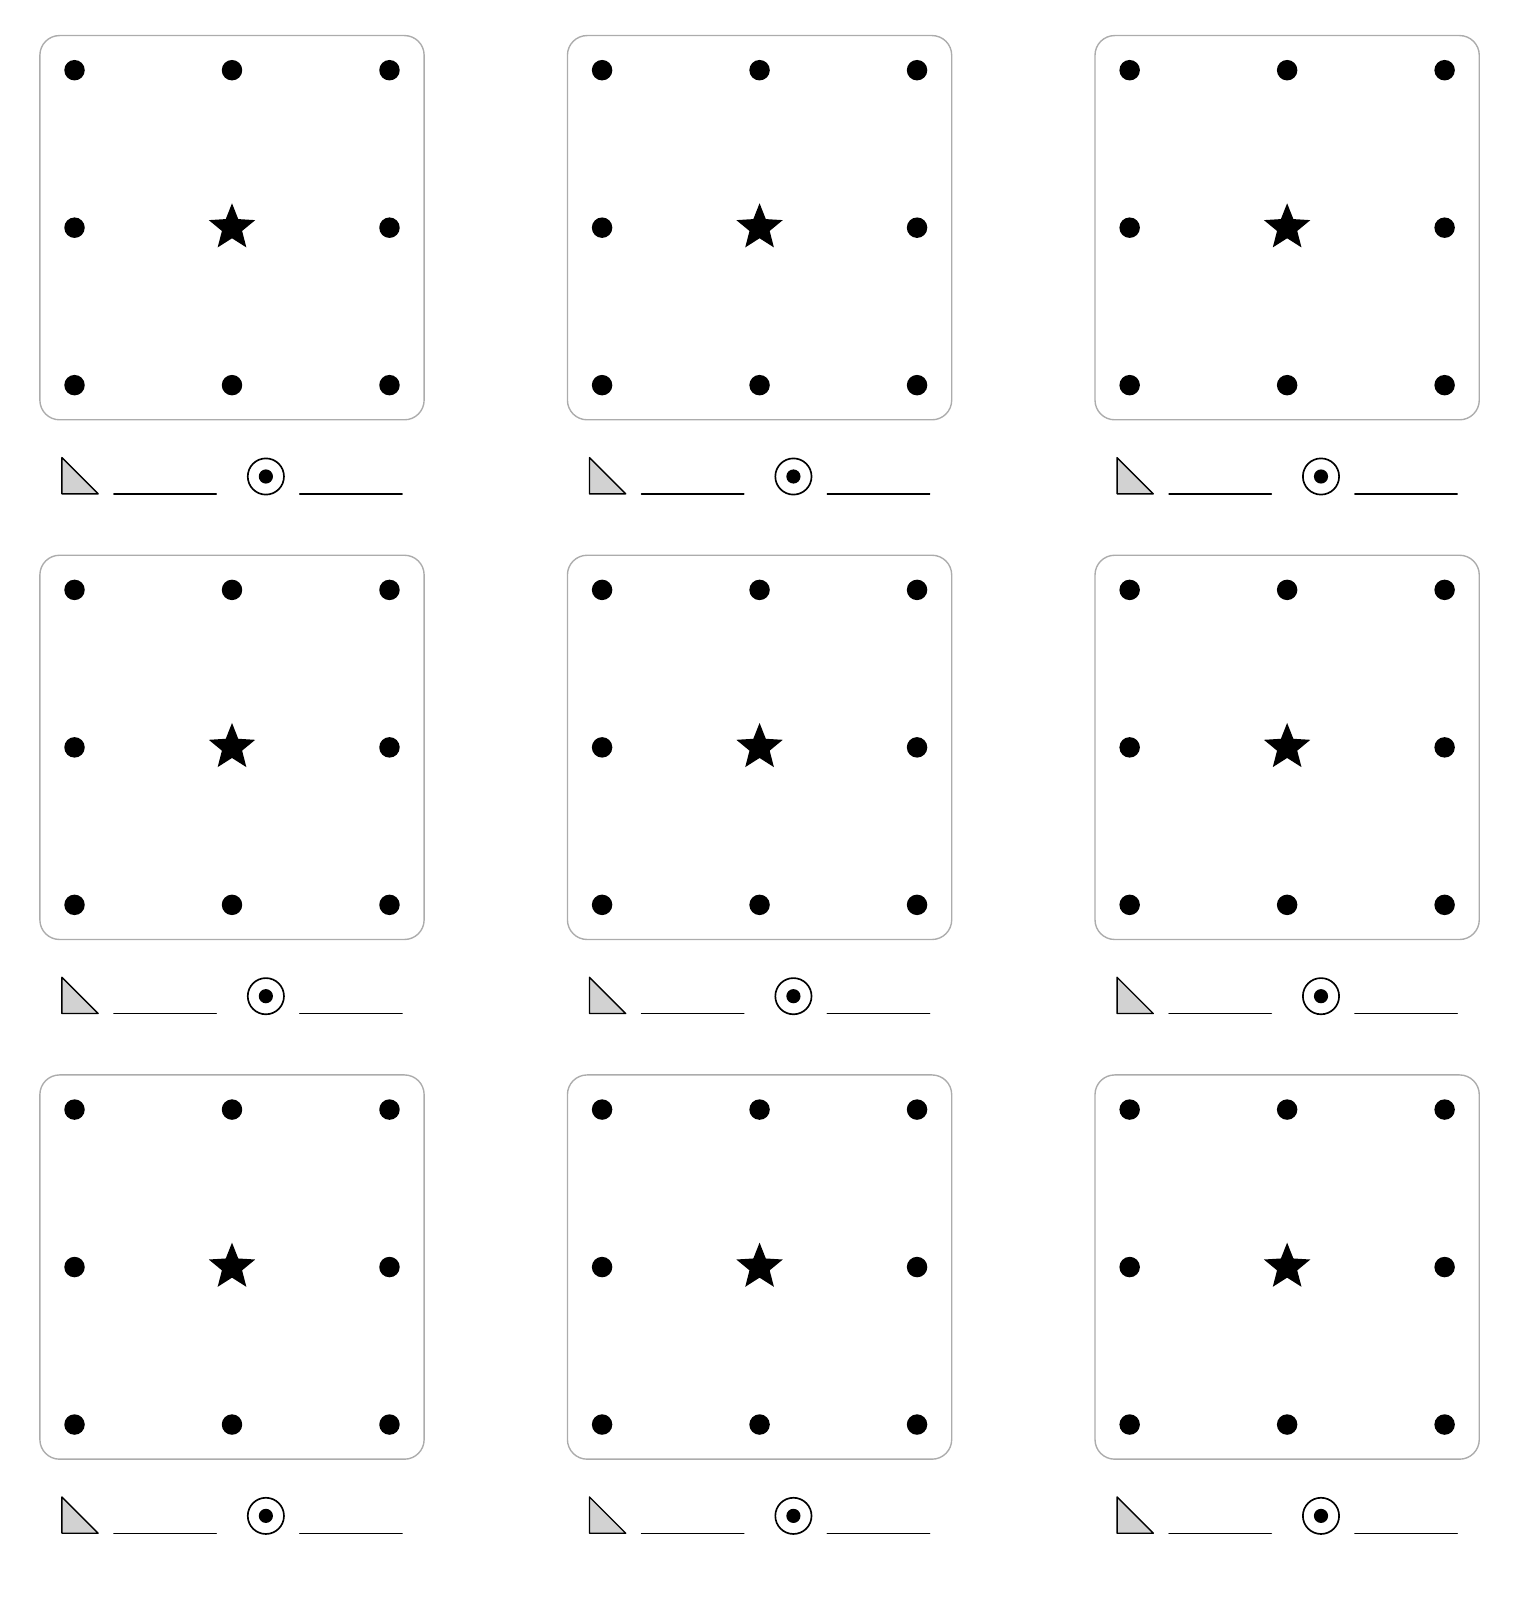
\begin{tikzpicture}[x=20mm,y=20mm]
  \useasboundingbox (0,-9.75) rectangle (9.295,0.05);
  \foreach \c in {0,1,2}{
    \foreach \r in {0,1,2}{
      \pgfmathsetmacro{\xl}{0.2975+\c*3.35}
      \pgfmathsetmacro{\yb}{-2.22-\r*3.3}
      \board{\xl}{\yb}{3}{3}
      \stardot{\xl+1,\yb+1}
      \recHC{\xl+1}{\yb-0.58}
    }
  }
\end{tikzpicture}

\newpage
% ============================== PAGE 6 ==============================
\prob{6} Make a shape with both stars inside, using as few pieces as you can.

\vspace{6mm}
\noindent\begin{tikzpicture}[x=20mm,y=20mm]
  \useasboundingbox (0,-0.25) rectangle (9.295,4.25);
  \board{2.1475}{0}{6}{5}
  \stardot{4.1475,2}
  \stardot{5.1475,2}
\end{tikzpicture}

\newpage
% ============================== PAGE 7 ==============================
\prob{7} Make a shape from eight halves with fewer dots on its outline than
this square.

\vspace{6mm}
\noindent
\begin{tikzpicture}[x=20mm,y=20mm]
  \useasboundingbox (0,-0.25) rectangle (9.295,2.2);
  \begin{scope}[shift={(3.6475,0)}]
    \fill[\shapefill] (0,0) rectangle (2,2);
    % the eight halves
    \draw[line width=0.6pt,gray!70] (0,0) -- (2,2) (1,0) -- (2,1) (0,1) -- (1,2)
      (1,0) -- (1,2) (0,1) -- (2,1);
    \draw[line width=1.3pt] (0,0) rectangle (2,2);
    \grid{0}{0}{3}{3}
    \foreach \x/\y in {0/0,1/0,2/0,2/1,2/2,1/2,0/2,0/1}{\cmark{\x,\y}}
    \bmark{1,1}
  \end{scope}
\end{tikzpicture}

\vspace{10mm}
% two boards of 4 x 5 dots, well apart so they do not read as one grid
\noindent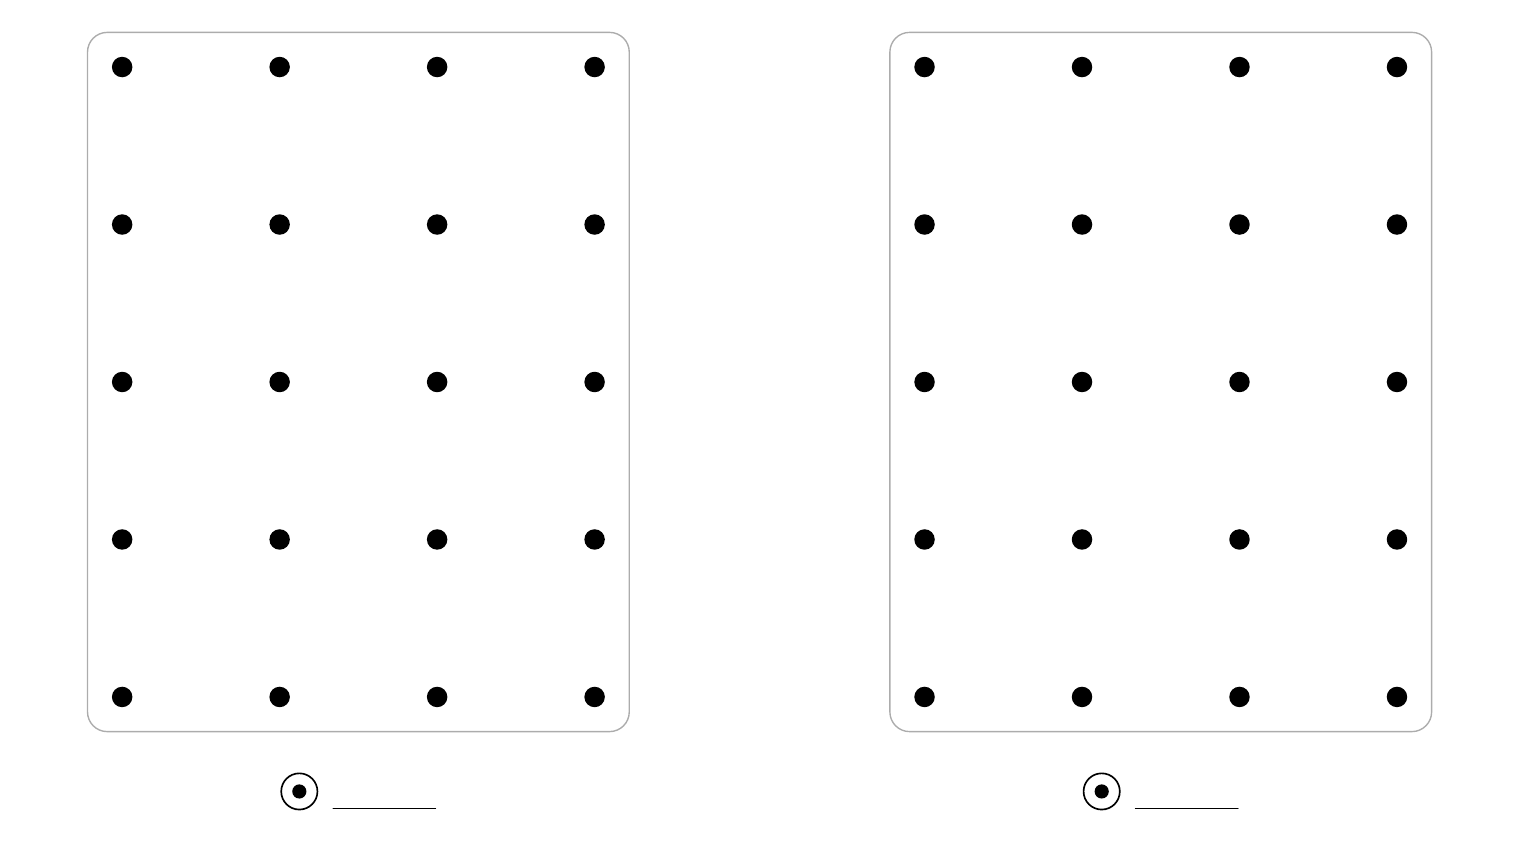
\begin{tikzpicture}[x=20mm,y=20mm]
  \useasboundingbox (0,-0.85) rectangle (9.295,4.25);
  \board{0.6}{0}{4}{5}
  \recC{2.1}{-0.6}
  \board{5.695}{0}{4}{5}
  \recC{7.195}{-0.6}
\end{tikzpicture}

\end{document}
